\documentclass[dvipsnames,crop=true]{standalone}
\usepackage{tikz}
\usepackage{amsmath}
\usetikzlibrary{calc,external,positioning}
\begin{document}

  \tikzsetnextfilename{generations}

  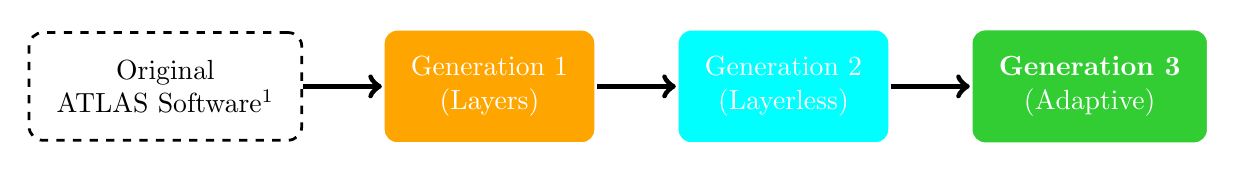
\begin{tikzpicture}[scale=1.0,line width=1pt]

    \tikzstyle{every node}=[rounded corners=5pt,draw,rectangle,inner sep=10pt,align=center]

    \node[dashed] (atlas) {
      Original\\
      ATLAS Software$^{\text{1}}$
    };

    \begin{scope}[white]
      \node[right=of atlas,fill=Orange] (gen1) {
        Generation 1 \\
        (Layers)
      };

      \node[right=of gen1,fill=Cyan] (gen2) {
        Generation 2 \\
        (Layerless)
      };

      \node[right=of gen2,fill=LimeGreen] (gen3) {
        \textbf{Generation 3} \\
        (Adaptive)
      };
    \end{scope}

    \begin{scope}[->,line width=2pt]
      \draw (atlas) -- (gen1);
      \draw (gen1) -- (gen2);
      \draw (gen2) -- (gen3); 
    \end{scope}

  \end{tikzpicture}

\end{document}
